\chapter{Design}
This chapter provides a representation of efforts one must face to make a jump from dry theoretical models to a virtually real product.

\section{On a quest to perfect parameters}
Our journey begins with a necessity to define restrictions of the problem. Intended environment would be a 4K cryogenic chamber (figure \ref{fig:4K_chamber}), which imposes dimensions restrictions. Ion trap requires a defined frequency for successful confinement of ions and has a capacitance. Summarized restrictions can be found in the table \ref{tbl:restrictions}.

\begin{table}[h]
\centering
\begin{tabular}{| l | r |}
	\hline
	Parameter & Value \\
	\hline \hline
	$L_{max}$ & 60 mm \\
	\hline
	$\omega_0$ & 40 MHz \\
	\hline
	$C_{trap}$ & 10--20 pF \\
	\hline
\end{tabular}	
\caption{Restrictions of a system}
\label{tbl:restrictions}
\end{table}

\subsection{First iteration}
Siverns' model \cite{Siverns2012} is dependent on outcomes from Macalpine's model \cite{Macalpine2000} thus one needs to find these beforehand. Exact value of a trap's capacitance is unknown at the moment of calculations so it was decided to use and compare values from a following set of capacitances: $C_{trap} = [10, 15, 20]\text{ pF}$. Modified Macalpine's model found in the appendix \ref{chapter:macalpine_code} also predicts resonant frequency fix when connecting a capacitor. Unloaded frequency needed to be varied until loaded frequency equals target frequency. Results are provided in the table \ref{tbl:macalpine}, naming is consistent with \cite{Macalpine2000}.

\begin{table}[h]
\centering
\begin{tabular}{| l | r | r | r |}
	\hline
	Parameter & \multicolumn{3}{r |}{Value} \\
	\hline \hline
	$C_{trap}$, pF & 10 & 15 & 20 \\
	\hline
	$B$, mm (length of a shield) & \multicolumn{3}{r |}{60.0} \\
	\hline
	$D$, mm (diameter of a shield) & \multicolumn{3}{r |}{45.0} \\
	\hline
	$b$, mm (length of a coil) & \multicolumn{3}{r |}{37.1} \\
	\hline
	$N_{t}$ (number of turns) & 11.0 & 9.2 & 8.1 \\
	\hline
	$d_0$, mm (diameter of a wire) & 1.7 & 2.0 & 2.3 \\
	\hline
	$\tau$, mm (pitch of a helix) & 3.4 & 4.0 & 4.6 \\
	\hline
	$f_0$, MHz (unloaded frequency) & 97.0 & 116.0 & 132.8 \\
	\hline
	$Q$ (unloaded quality factor) & 873.2 & 954.8 & 1022.4 \\
	\hline
\end{tabular}
\caption{Joint output of the appendix \ref{chapter:macalpine_code}}
\label{tbl:macalpine}
\end{table}

\subsection{Precise fit}
After defining an approximate region of our interest we can proceed to calculations utilizing Siverns' model \cite{Siverns2012} with implementation provided in the appendix \ref{chapter:siverns_code}. Volume requirements were also better clarified making the goal to get the best quality factor by varying coil's parameters. Updated restrictions can be found in the table \ref{tbl:restrictions_siverns}. One could argue that all values of $d_0$ are lower than recommended in \cite{Siverns2012} thickness of 5 mm. This is true and additional measures to handle it can be found in the section X.

\begin{table}[h]
\centering
\begin{tabular}{| l | r | r | r |}
	\hline
	Parameter & \multicolumn{3}{r |}{Value} \\
	\hline \hline
	$C_{trap}$, pF & 10 & 15 & 20 \\
	\hline
	$B$, mm (length of a shield) & \multicolumn{3}{r |}{56.0} \\
	\hline
	$D_{max}$, mm (max diameter of a shield) & \multicolumn{3}{r |}{38.0} \\
	\hline
	$d_0$, mm (diameter of a wire) & 1.7 & 2.0 & 2.3 \\
	\hline
	$\tau$, mm (pitch of a helix) & 3.4 & 4.0 & 4.6 \\
	\hline
\end{tabular}
\caption{Restrictions for the Siverns' model}
\label{tbl:restrictions_siverns}
\end{table}

Fixed values of the table \ref{tbl:restrictions_siverns} allow us to independently change 2 remaining parameters --- diameter of a shield and diameter of a coil. Appendix's \ref{chapter:siverns_code} output of $Q$ values is provided in the figures \ref{fig:q_plot_10}, \ref{fig:q_plot_15}, \ref{fig:q_plot_20}. By selecting a point in a $\{d, \gamma = d / D\}$ space that maximizes $Q$ for a set of $C_{trap}$ values we get final parameters of an RF resonator as defined in the table \ref{tbl:final_parameters}.
\clearpage
\begin{figure}[!h]
\centering
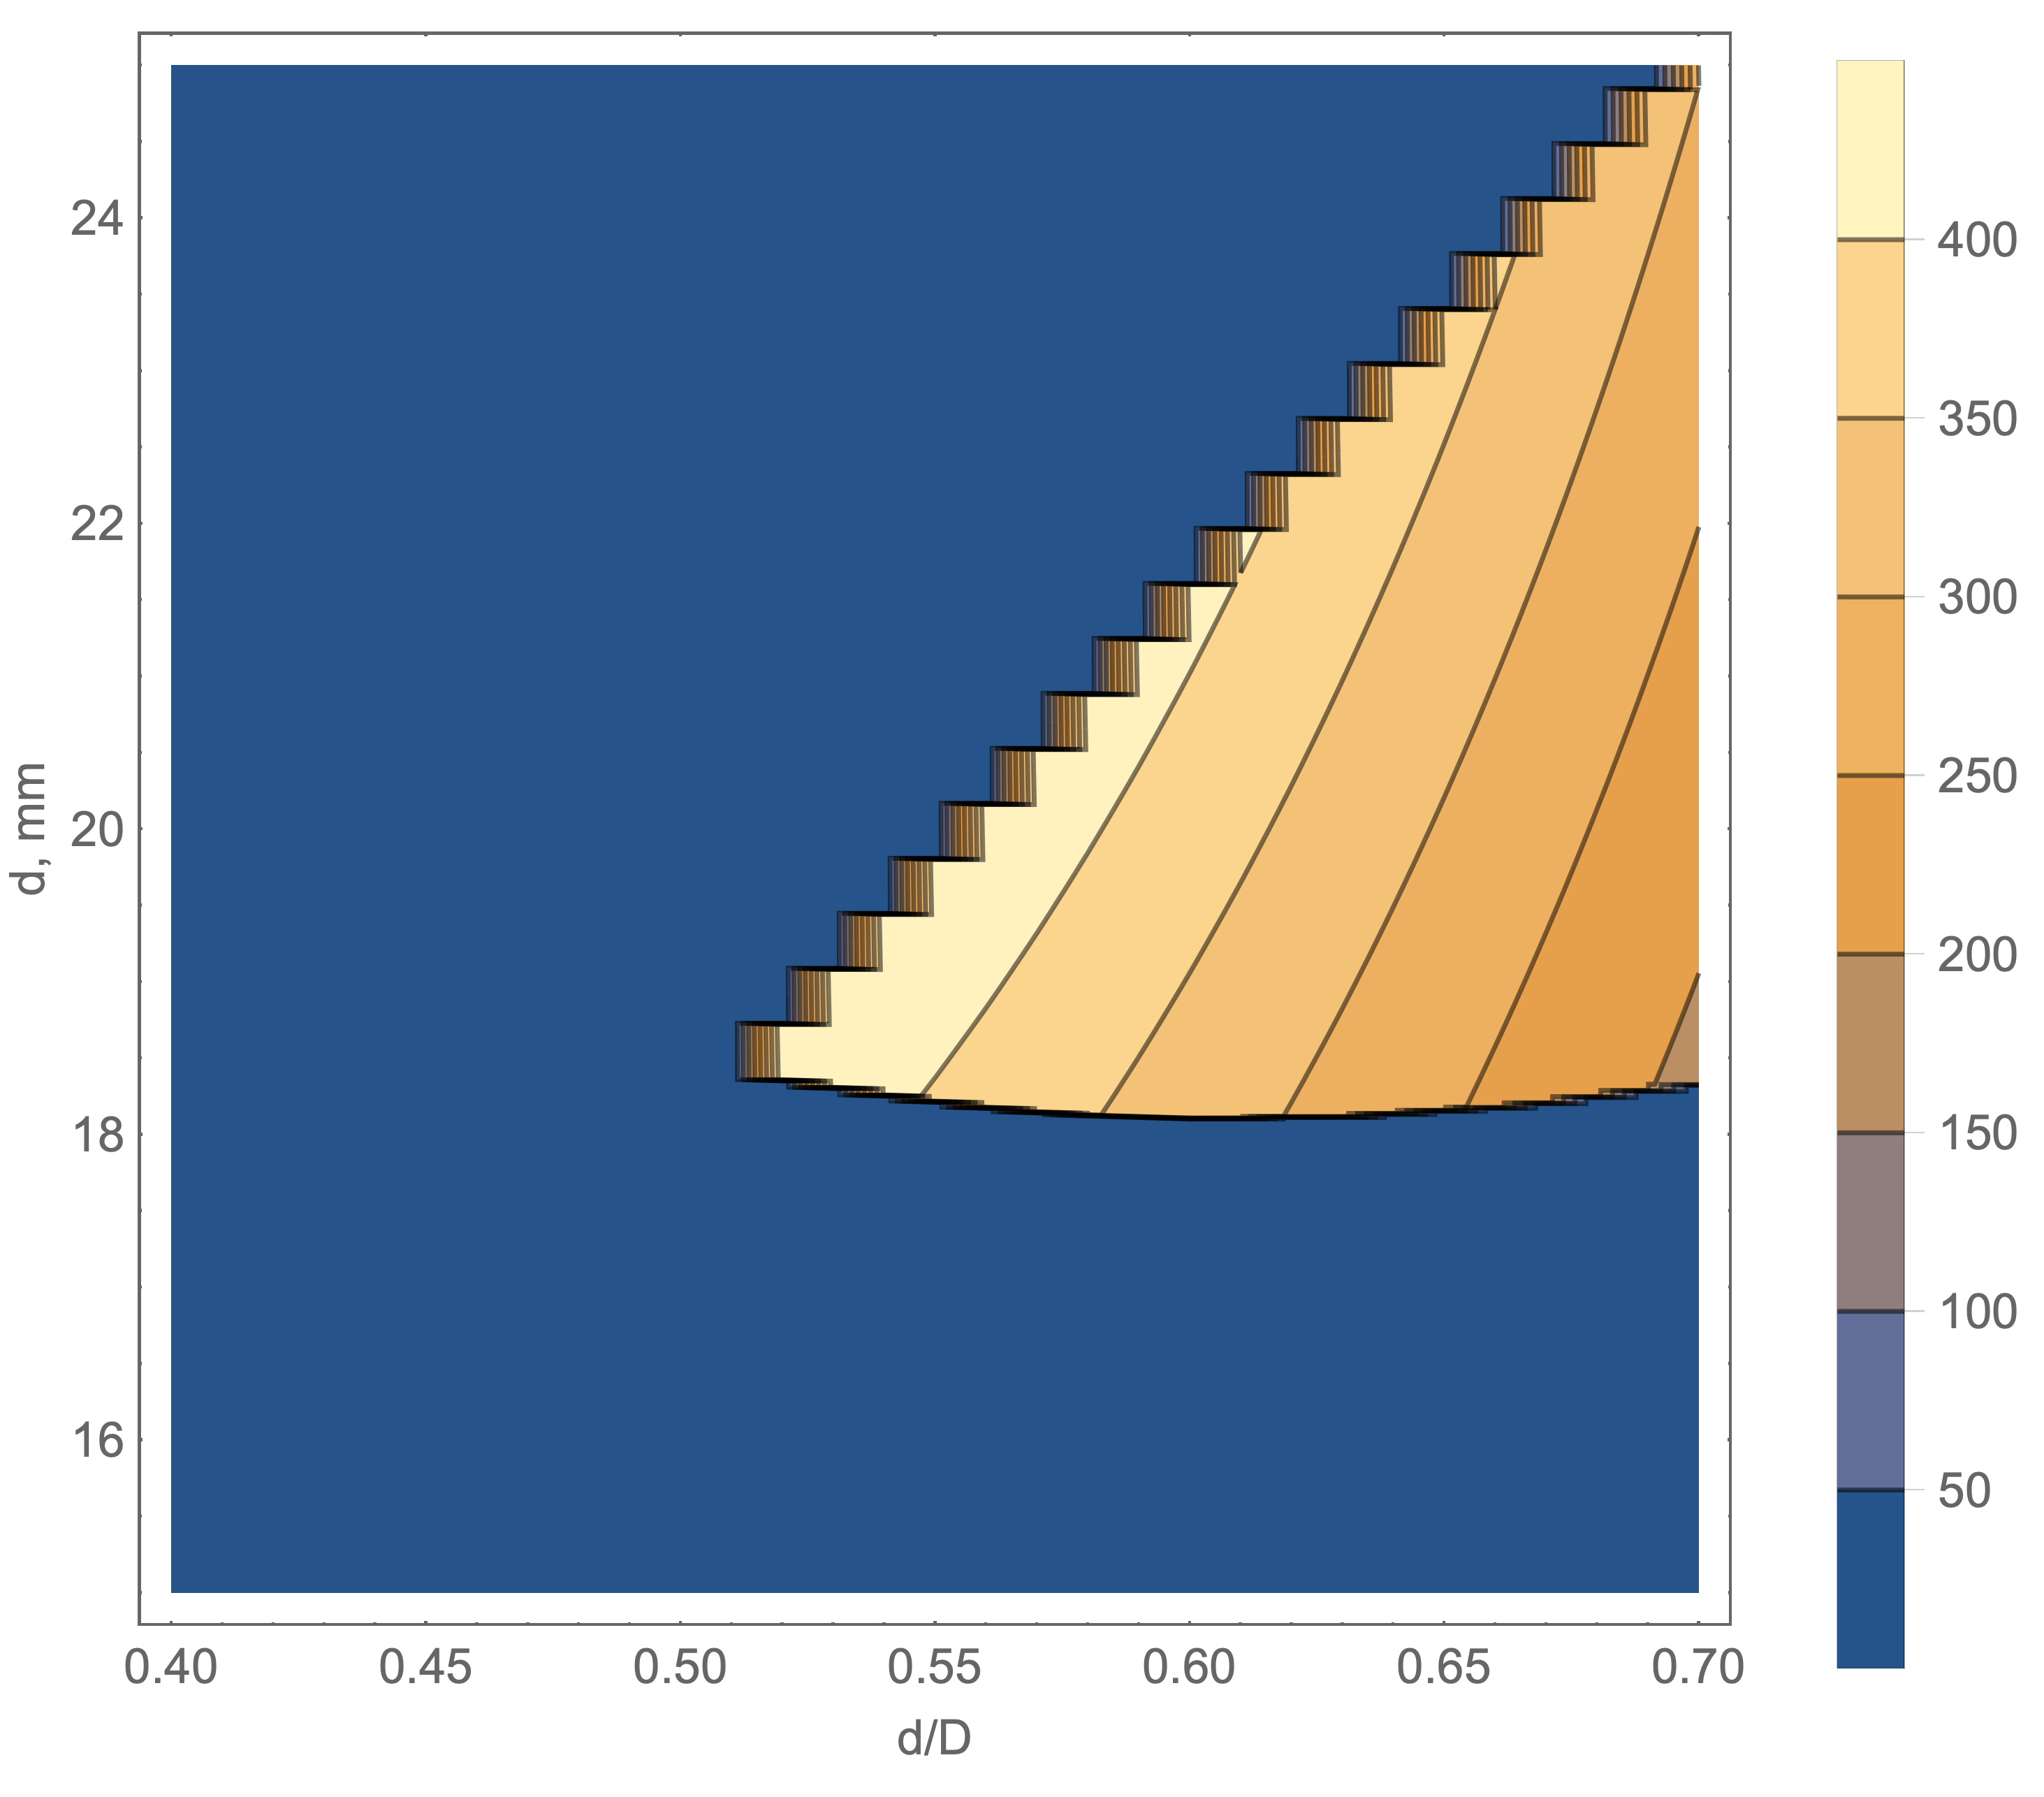
\includegraphics[width=.78\textwidth]{images/q_plot_siverns_tex_10}
\caption{$Q$ plot for $C_{trap} = 10$ pF}
\label{fig:q_plot_10}
\end{figure}
\begin{figure}[!h]
\centering
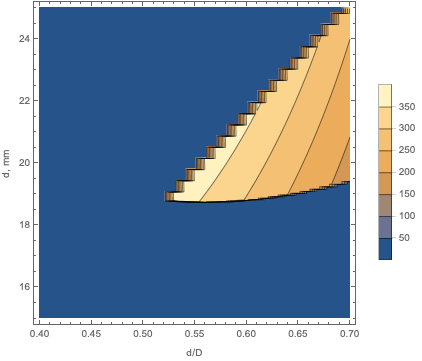
\includegraphics[width=.78\textwidth]{images/q_plot_siverns_tex_15}
\caption{$Q$ plot for $C_{trap} = 15$ pF}
\label{fig:q_plot_15}
\end{figure}
\begin{figure}[!h]
\centering
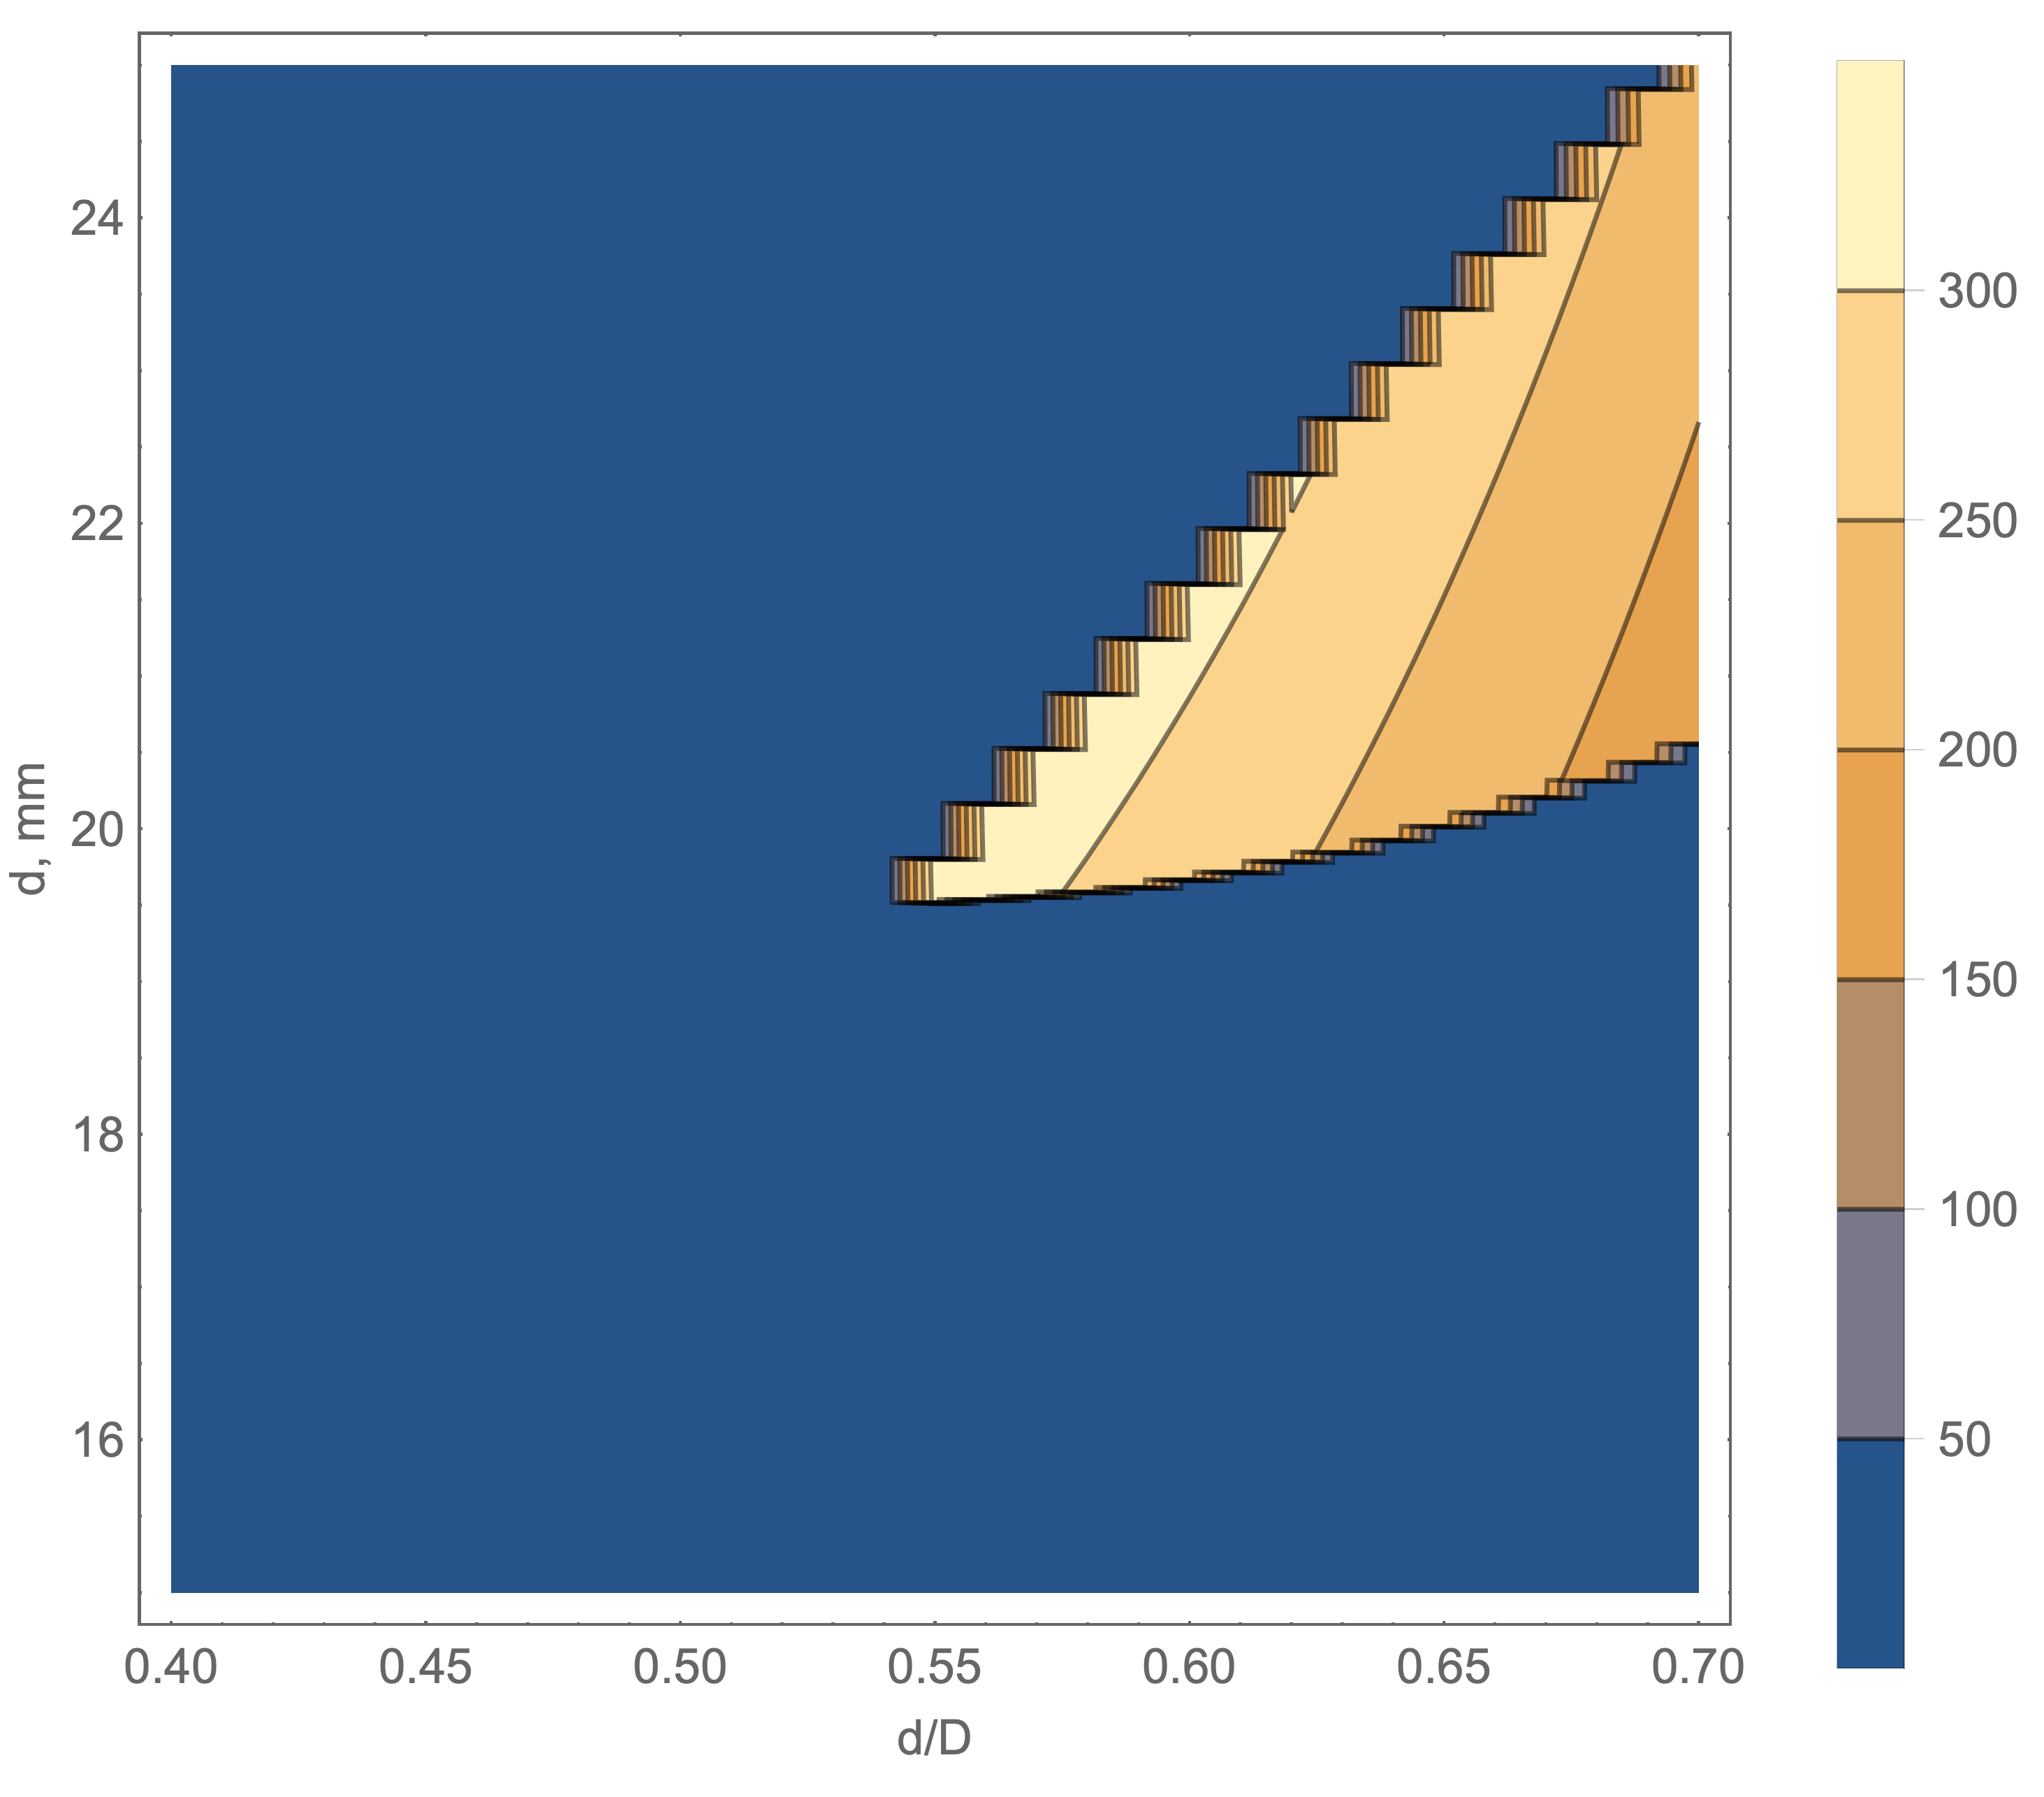
\includegraphics[width=.78\textwidth]{images/q_plot_siverns_tex_20}
\caption{$Q$ plot for $C_{trap} = 20$ pF}
\label{fig:q_plot_20}
\end{figure}
\begin{table}[h]
\centering
\begin{tabular}{| l | r |}
	\hline
	Parameter & Value\\
	\hline \hline
	$B$, mm (length of a shield) & 56.0 \\
	\hline
	$D$, mm (diameter of a shield) & 34.5 \\
	\hline
	$d$, mm (diameter of a coil) & 19.0 \\
	\hline
	$b$, mm (length of a coil) & 40.0 \\
	\hline
	$N_{t}$ (number of turns) & 10.0 \\
	\hline
	$d_0$, mm (diameter of a wire) & 2.0 \\
	\hline
	$\tau$, mm (pitch of a helix) & 4.0 \\
	\hline
\end{tabular}
\caption{Final parameters of an RF resonator}
\label{tbl:final_parameters}
\end{table}

\section{Shining in 3D}